\section{Research and Software Development Methodologies}
\label{sec:software-development-methodology}

As discussed in Chapter \ref{chap:new-ideas}, the software development methodology followed during implementation was agile, chosen due to its support for rapid iteration and flexibility, allowing previously completed areas to be revisited if issues are encountered, for example.
Figure \ref{fig:agile-development-process} below provides an overview of the agile devleopment process:

\begin{figure}[H]
    \centering
    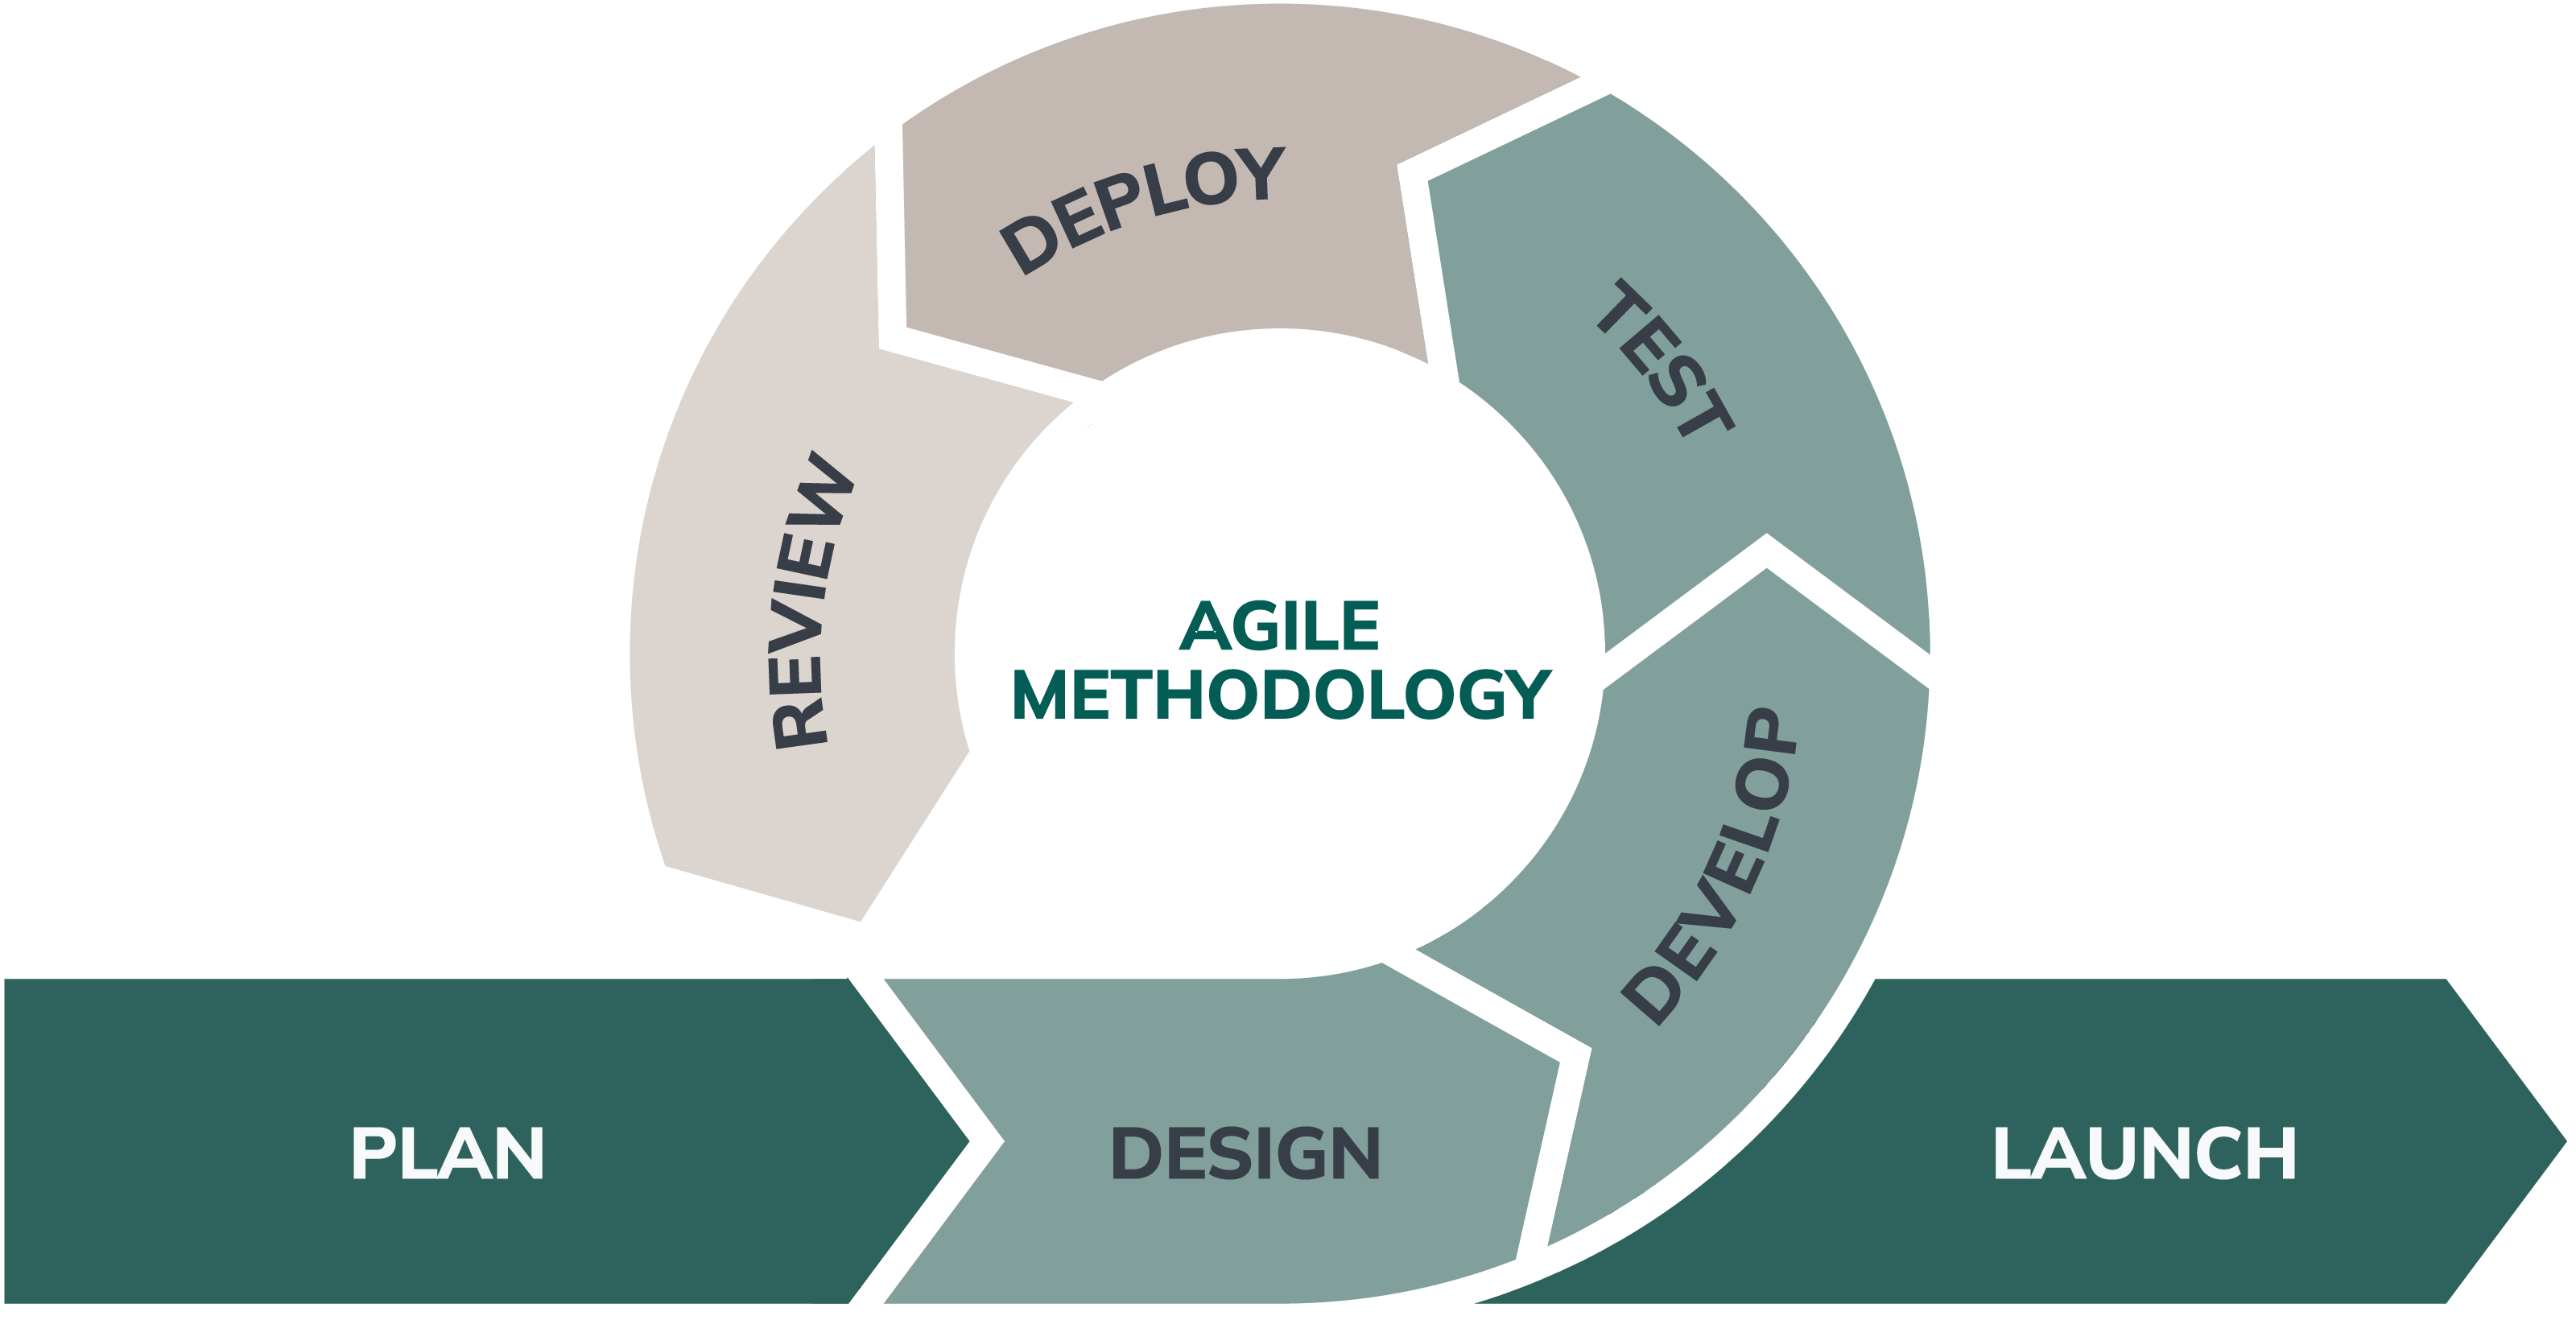
\includegraphics[width=0.8\textwidth]{assets/agile.png}
    \caption{Agile Software Development Process}
    \label{fig:agile-development-process}
\end{figure}

While software development \ref{sec:implementation} was completed following the agile methodology, the overall research project is structured as follows:

\begin{enumerate}
    \item \textbf{Research}: The current state-of-the-art in \ac{pacs}, biometrics, and \ac{gr} is researched, with comparisons made between technologies to identify security and usability-related trade-offs.
    \item \textbf{Survey}: A survey was conducted to gather feedback from the public (potential users) on their perceptions and openness to \ac{gr} technology in the context of access control.
    \item \textbf{Proposal}: A 'new idea' --- the software deliverable of this project --- is proposed, with a high-level overview of what the system will do, with aims, objectives, and requirements defined.
    \item \textbf{Design}: The system architecture is designed based on the proposal, with a general understanding gathered of how the problem will be tackled, and how components will operate and interact with each other and external entities.
    \item \textbf{Implementation}: The system is implemented, with decisions made on what technologies to use, and the exact way in which the system will be constructed. Following the agile methodology, this happens incrementally.
    \item \textbf{Testing}: The system is tested based on functionality and performance requirements defined in the proposal, relating to project objectives.
    \item \textbf{Evaluation}: The final solution is evaluated based on the aims and objectives defined in the proposal, with a focus on security and usability. A feasibility study is also conducted to determine if the system is ready for deployment in a real-world scenario.
\end{enumerate}

The following sections outline the software and hardware technologies used when implementing the solution, followed by the design, and implementation documentation.
